\section{Radiative Corrections II}

\subsection{The Goal: One-Loop Correction to the Electron Dipole Moment}
Today we do the calculation to determine the correction to the electron dipole moment:
\begin{equation}
    \mu = \frac{e}{2m}(1 + \frac{\alpha}{2\pi} + O(\alpha^2))
\end{equation}
with:
\begin{equation}
    \frac{\alpha}{2\pi} = \frac{1}{2\pi}\frac{e^2}{2\pi} = \frac{1}{2\pi}\frac{e^2}{4\pi \e_0\hbar c} = 0.00116\ldots
\end{equation}
These are the promised 5 extra digits of precision that we obtain by going to one loop.

To find this, we will evaluate the correction to the vertex function:
\begin{equation}
    \delta \avg{j^\mu_p \psi \bar{\psi}_{p'}}_{\text{amp}} = \frac{1}{G(p + p')}\delta\avg{j^\mu_p \psi \bar{\psi}_{p'}} \frac{1}{G(p')}
\end{equation}
When the electron is on-shell, i.e. $p'^2 = -m^2 = (-\v{p} - \v{p}')^2$ and we sandwich the expression with $\bar{u}(\v{p} + \v{p}') \ldots u(\v{p}')$,  this has the general form:
\begin{equation}
    \delta \avg{j^\mu_p \psi \bar{\psi}_{p'}}_{\text{amp}} = \gamma^\mu F_1(\frac{p^2}{m^2}) + iS^{\mu\nu}\frac{p_\nu}{m}F_2(\frac{p^2}{m^2}) \stackrel{\text{free}}{\to} \gamma^\mu
\end{equation}
We will be particularly interested in:
\begin{equation}
    \mu = \frac{e}{2m}\left(1 + F_2(0)\right)
\end{equation}

\subsection{Which diagrams contribute?}
The diagram that produces $F_2$ is the one that is not a self-energy correction:
\begin{center}
    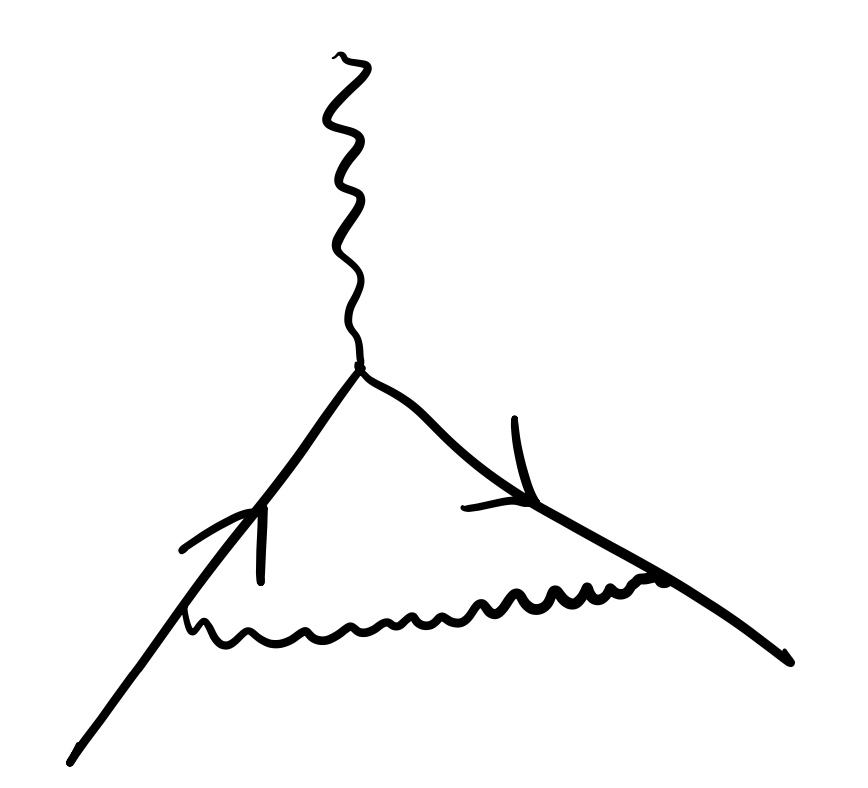
\includegraphics[scale=0.35]{Lectures/Images/lec10-relevantdiagram.png}
\end{center}

The self-energy correction to the dirac propagator only gives $\gamma^\mu$, as it renormalizes $G(p') = \slashed{p}'(\ldots) + \II(\ldots)$. The identity term gives the $\gamma^\mu$ and the first term (when sandwiching with the $u$s, which are solutions to the dirac equation and thus $(\slashed{q} + m)u(\v{q}) = 0 = \bar{u}(\v{q})(\slashed{q} + m)$) gives $-m$.
\begin{center}
    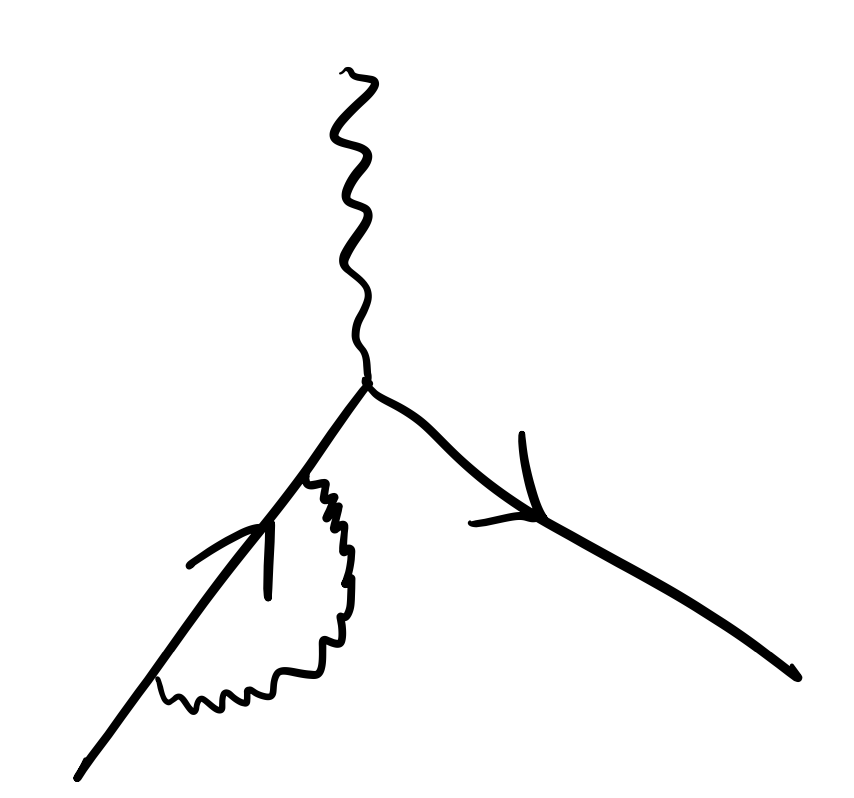
\includegraphics[scale=0.35]{Lectures/Images/lec10-diracselfE.png}
\end{center}
The self-energy correction to the photon also only gives $\gamma^\mu$. It renormalizes $G_{\mu\nu}(p) = \eta_{\mu\nu}(\ldots) + p_\mu p_\nu (\ldots)$, the $\eta_{\mu\nu}$ piece giving us $\gamma^\mu$, the $p_\mu p_\nu$ piece giving zero (why? $\bar{u}(\v{p} + \v{p}')\slashed{p})u(\v{p}') = 0$, because we can write $\slashed{p} = \slashed{p} + \slashed{p}' - \slashed{p}'$ and then acting on the left/right we get $\pm m$ which cancel. 
\begin{center}
    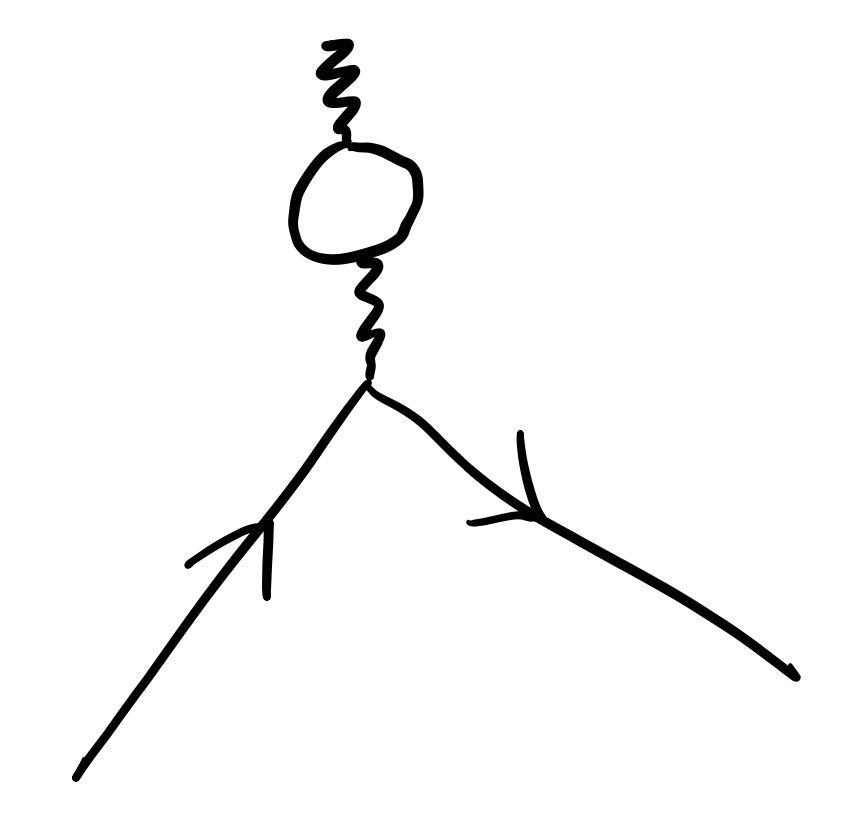
\includegraphics[scale=0.35]{Lectures/Images/lec10-photonselfE.png}
\end{center}
These diagrams will matter for other things - when we look at the renormalization and $\beta$ function of QED they are important (and you will look at the second diagram in the homework). But, for the $e^{-}$ dipole moment we only need consider the one diagram. Unfortunately, it is the most complicated, namely because we have a loop with three propagators. 

\subsection{Evaluating the 1-loop correction}
Graphically, the diagram (in momentum space) looks like:
\begin{center}
    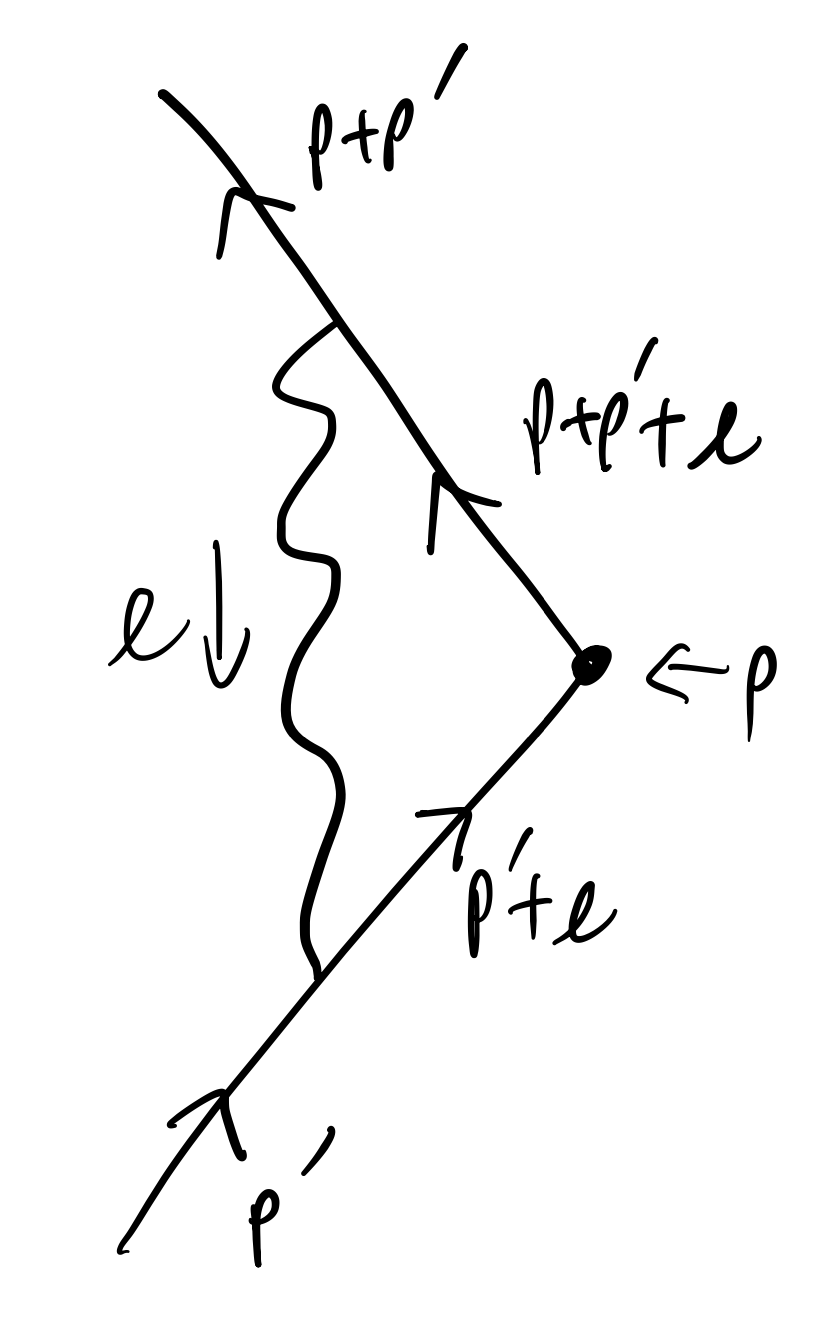
\includegraphics[scale=0.35]{Lectures/Images/lec10-momenta.png}
\end{center}

So our correction is of the form:
\begin{equation}
    \delta \avg{j^\mu_p \psi \bar{\psi}_{p'}} = \frac{i^2}{2}\avg{j^\mu_p \psi \bar{\psi}_{p'}(S_{\text{int}})^2} = -\frac{e^2}{2}\avg{(\bar{\psi}\gamma^\mu \psi)_p \left(\int_{x_1}A_\alpha \bar{\psi}\gamma^\alpha \psi \right)\left(\int_{x_2}A_\beta \bar{\psi}\gamma^\beta \psi \right)\psi \bar{\psi}_{p'}}
\end{equation}
We contract the $\psi$ in the current with $\bar{\psi}$ in the $x_1$ integral (2 possible choices, so factor of 2), and then $\bar{\psi}$ in the current with $\psi$ in the $x_2$ integral (we get a $-$ sign), then remaining $\bar{\psi}$ in $x_2$ with the $\psi$ on the right (another $-1$ sign) and $\psi$ in the $x_1$ with $\bar{\psi}$ on the right. When the smoke clears, we have:
\begin{equation}
    \delta \avg{j^\mu_p \psi \bar{\psi}_{p'}} = -e^2\int \frac{d^4l}{(2\pi)^4}G(p + p')\gamma^\beta G(p + p' + l)\gamma^\mu G(p' + l)\gamma^\alpha G(p') G_{\alpha\beta}(l)
\end{equation}
with the last term being the photon propagator (we have 4 dirac propagators and 1 photon propagator). We amputate this to make our lives simpler, which removes the $G(p + p')$ and $G(p')$:
\begin{equation}
    \delta \avg{j^\mu_p \psi \bar{\psi}_{p'}}_{\text{amp}} = -e^2\int \frac{d^4l}{(2\pi)^4}\gamma^\beta G(p + p' + l)\gamma^\mu G(p' + l)\gamma^\alpha G_{\alpha\beta}(l)
\end{equation}
Inserting our known expressions for the propagators (allowing ourselves to gauge fix with $\xi = 1$ such that we just have $G_{\alpha\beta}(l) = \frac{-i}{l^2}\eta_{\alpha\beta}$)
\begin{equation}
    \delta \avg{j^\mu_p \psi \bar{\psi}_{p'}}_{\text{amp}} = -e^2\int_l \gamma^\beta \frac{-i(\slashed{p} + \slashed{p}' + \slashed{l} - m)}{(p + p' + l)^2 + m^2}\gamma^\mu \frac{-i(\slashed{p}' + \slashed{l} - m)}{(p' + l)^2 + m^2}\gamma^\alpha \frac{-i}{l^2}\eta_{\alpha\beta}
\end{equation}
we will treat this in the usual way using Feynman parameters - with two propagators we used 1 Feynman parameter, with three propagators we shall use 2. We will use the identity (see Srednicki for the $n$-propagator version):
\begin{equation}
    \frac{1}{ABC} = 2\int_0^1 dx \int_0^{1-x}dy \frac{1}{[xA + yB + (1-x-y)C]^3}
\end{equation}
where we integrate over a triangle in the $xy$ plane. 
\begin{center}
    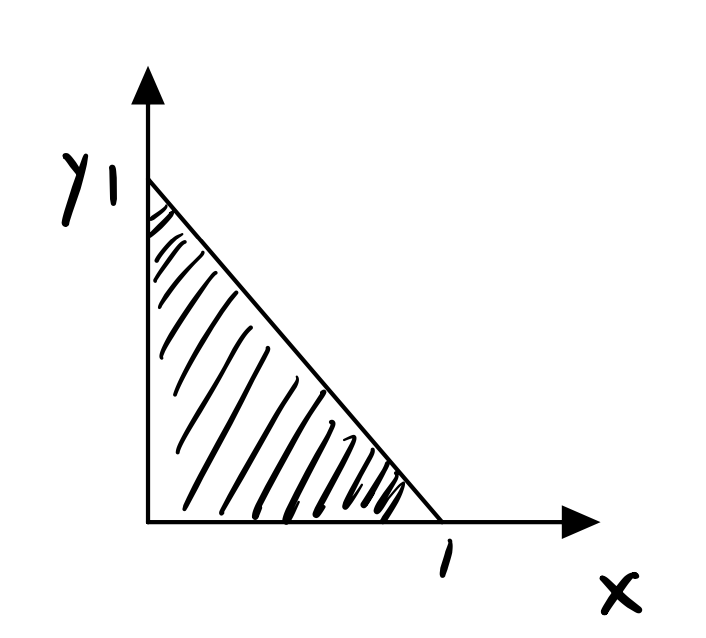
\includegraphics[scale=0.35]{Lectures/Images/lec10-triangle.png}
\end{center}
Applying this identity:
\begin{equation}
    \delta \avg{j^\mu_p \psi \bar{\psi}_{p'}}_{\text{amp}} = -2e^2\int_{xy}\int_l  \frac{-i(\slashed{p} + \slashed{p}' + \slashed{l} - m)\gamma^\mu \cdot -i(\slashed{p}' + \slashed{l} - m)\gamma^\alpha \cdot -i\eta_{\alpha\beta}}{l^2 + m^2(x+y) + p'^2x + (p + p')^2y + 2lp'x + 2l(p + p')y}
\end{equation}
Now writing the denominator as:
\begin{equation}
    \left([l + p'y + (p + p')x]^2 + m^2(x + y) + p'^2y + (p + p')^2x - [p'y + (p+p')x]^2\right)^3
\end{equation}
Renaming $[l + p'y + (p + p')x] = q$ and $\Delta(x, y) = m^2(x + y) + p'^2y + (p + p')^2x - [p'y + (p+p')x]^2$, we have:
\begin{equation}
    \delta \avg{j^\mu_p \psi \bar{\psi}_{p'}}_{\text{amp}} = -2ie^2\int_q \int_{xy}\frac{\gamma^\alpha((1-x)(\slashed{p} + \slashed{p}') - y\slashed{p}' + \slashed{q} -m)\gamma^\mu((1-y)\slashed{p}' - x(\slashed{p}+\slashed{p}') + \slashed{q} - m)\gamma_\alpha}{[q^2 + \Delta]^3}
\end{equation}
we have made the numerator terrible at expense of making the denominator simple, but the odd-in-q parts will integrate to zero via parity symmetry.

\subsection{UV divergent part}
Does this integral have a UV divergence? Indeed, it goes as $\sim \int d^4q \frac{q^2}{q^6}$ which is a logarithmic divergence. In more detail, the UV divergent part looks like:
\begin{equation}
    \delta \avg{j^\mu_p \psi \bar{\psi}_{p'}}_{\text{amp}} = -2ie^2\int_{xy}\int_q\frac{\gamma^\alpha \slashed{q}\gamma^\mu \slashed{q}\gamma_\alpha}{[q^2 + \Delta]^3}
\end{equation}
and now using the identity:
\begin{equation}
    \gamma^\alpha \slashed{p}\slashed{k}\slashed{q}\gamma_\alpha = 2\slashed{q}\slashed{k}\slashed{p}
\end{equation}
we have (taking the derivative w.r.t. $k_\mu$) and the case where $p = q$:
\begin{equation}
    \gamma^\alpha \slashed{q}\gamma^\mu \slashed{q}\gamma_\alpha = 2\slashed{q}\gamma^\mu \slashed{q} = 2\slashed{q}(-\slashed{q}\gamma^\mu - 2q^\mu) = 2q^2\gamma^\mu - 4\slashed{q}q^\mu
\end{equation}
Thus:
\begin{equation}
    \delta \avg{j^\mu_p \psi \bar{\psi}_{p'}}_{\text{amp}} = -4ie^2\int_{xy}\int_q\frac{q^2\gamma^\mu - 2q^\mu q^\nu \gamma_\nu}{[q^2 + \Delta]^3} = -4ie^2\gamma_\nu \int_{xy}\int_q\frac{q^2\eta^{\mu\nu} - 2q^\mu q^\nu}{[q^2 + \Delta]^3}
\end{equation}
Since the integral is isotropic, we can replace the second term:
\begin{equation}
    q^\mu q^\nu = \eta^{\mu\nu}q^2\frac{1}{4}
\end{equation}
and so:
\begin{equation}
    \delta \avg{j^\mu_p \psi \bar{\psi}_{p'}}_{\text{amp}} = -2ie^2\gamma_\mu \int_{xy}\in_{q}\frac{q^2}{[q^2 + \Delta]^3}
\end{equation}
so, we notice that the entire UV divergent term is $\propto \gamma^\mu$ and as such does not enter the correction to the electron dipole moment. It will be relevant for renormalizing the electron charge. But, let's still compute this because we will still care about this when we study RG for QED. We recover the $-i\e$ in the denominator:
\begin{equation}
    \delta \avg{j^\mu_p \psi \bar{\psi}_{p'}}_{\text{amp}} = -2ie^2\gamma_\mu \int_{xy}\in_{q}\frac{q^2}{[q^2 + \Delta-i\e]^3}
\end{equation}
which shifts the poles of $q_0$ off the real axis, and we can choose an appropriate contour (see below)
\begin{center}
    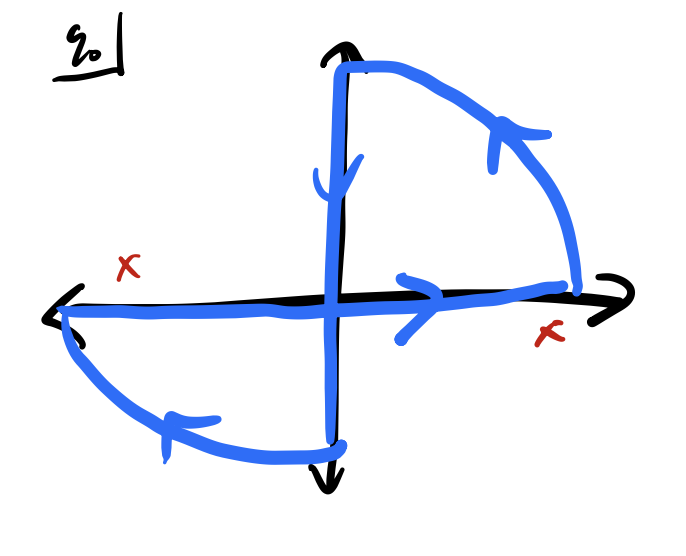
\includegraphics[scale=0.35]{Lectures/Images/lec10-contour.png}
\end{center}
which gives us the Wick rotation $q_0 \to iq_0^E$, allowing us to compute the (real) integral:
\begin{equation}
    \delta \avg{j^\mu_p \psi \bar{\psi}_{p'}}_{\text{amp}} = 2e^2\gamma^\mu \int_{xy}\int_{q_E}\frac{q^2}{[q^2 + \Delta]^3} = 2e^2\gamma^\mu \int_{xy}\frac{2\pi^2}{(2\pi)^4}\int_0^\infty dq \frac{q^5}{[q^2 + \Delta]^3} = \frac{e^2\gamma^\mu}{4\pi^2}
\end{equation}
In Wilsonian RG, we integrate $b\Lambda < q < \Lambda$ with $\Lambda \gg m, p, p', \Delta^{1/2}$, so we obtain:
\begin{equation}
    \delta \avg{j^\mu_p \psi \bar{\psi}_{p'}}_{\text{amp}} = -\frac{e^2\gamma^\mu}{4\pi^2}\int_{xy}\int_{b\Lambda}^\Lambda \frac{dq}{q} = \frac{e^2}{8\pi^2}\log(\frac{1}{b})\gamma^\mu
\end{equation}
where he $xy$ integral is now trivial and gives 1/2. This thus gives the renormalization of charge:
\begin{equation}
    \gamma^\mu(1 + \frac{e^2}{8\pi}\log(\frac{1}{b}))
\end{equation}
note there are other diagrams that contribute here, which we will need when we do RG. We did this with a cutoff here, but it is not a good idea to do here as it breaks gauge invariance. In the HW you will look at dimensional regularization. The $\log(\frac{1}{b})$ gets replaced with $-\frac{1}{\e}$ where $\e$ is the regulated dimension.

\subsection{Back to the electron dipole moment}
So, we found that the $O(q^2)$ term only matters when we do RG and not for the dipole moment. Further, the $O(q)$ terms go to 0 by $q \leftrightarrow -q$ symmetry. So, we can just set $q = 0$ and see what remains; after Wick rotation:
\begin{equation}
    \delta \avg{j^\mu_p \psi \bar{\psi}_{p'}}_{\text{amp}} = 2e^2\int_{xy}\int_q \frac{\gamma^\alpha((1-x)(\slashed{p} + \slashed{p}') - y\slashed{p}' - m)\gamma^\mu(\slashed{p}'(1-y) - x(\slashed{p} + \slashed{p}') - m)\gamma_\alpha}{[q^2 + \Delta]^3}
\end{equation}
Now the $q$-integral is easy because only the denominator has $q$ dependence:
\begin{equation}
    \int_q \frac{1}{[q^2 + \Delta]^3} = \frac{2\pi^2}{(2\pi)^4}\int_0^\infty \frac{dq q^3}{[q^2 + \Delta]^3} = \frac{1}{8\pi^2}\frac{1}{\Delta}\int_0^\infty \frac{ds s^3}{(s^2 + 1)^3} = \frac{1}{32\pi^2}\frac{1}{\Delta}
\end{equation}
So then:
\begin{equation}
    \delta \avg{j^\mu_p \psi \bar{\psi}_{p'}}_{\text{amp}} = \frac{e^2}{16\pi^2}\int_{xy}\frac{1}{\Delta}(\gamma^\alpha((1-x)(\slashed{p} + \slashed{p}') - y\slashed{p}' - m)\gamma^\mu(\slashed{p}'(1-y) - x(\slashed{p} + \slashed{p}') - m)\gamma_\alpha)
\end{equation}
Let's look at the numerator. We showed that it has to take the form:
\begin{equation}
    \bar{u}(\v{p}+ \v{p}') \ldots u(\v{p}') =  \bar{u}(\v{p}+ \v{p}')\gamma^\mu F_1(\frac{p^2}{m^2}) + iS^{\mu\nu}\frac{p_\nu}{m}F_2(\frac{p^2}{m^2})u(\v{p}')
\end{equation}
So, lets take this numerator and simplify this when we sandwich it via $u$s. Let's invoke the $\gamma$ matrix technology:
\begin{equation}
    \gamma^\alpha \slashed{p}\slashed{q}\gamma_\alpha = 4p\cdot q
\end{equation}
\begin{equation}
    \gamma^\alpha \slashed{p}\gamma_\alpha = 2\slashed{p}
\end{equation}
so then with $a = (1-x)(p + p') - yp'$, $b = (1-y)p' - y(p + p')$.
\begin{equation}\label{eq:lec10temp}
    \gamma^\alpha (\slashed{a} - m)\gamma^\mu (\slashed{b} - m)\gamma_\alpha = 2\slashed{b}\gamma^\mu \slashed{a} - 4(a^\mu + b^\mu)m + 2m^2\gamma^\mu
\end{equation}
we can drop the $\gamma^\mu$ terms (again these do not contribute to the $F_2$ term). Now using the EOM of the spinors:
\begin{equation}
    (\slashed{p}' + m)u(\v{p}') = 0 = \bar{u}(\v{p} + \v{p}')(\slashed{p} + \slashed{p}' + m)
\end{equation}
The first term of Eq. \eqref{eq:lec10temp} becomes:
\begin{equation}
    \begin{split}
        2\slashed{b}\gamma^\mu \slashed{a} &= 2((1-y)\slashed{p}' + xm)\gamma^\mu ((1 - x)(\slashed{p} + \slashed{p}') + ym) 
        \\ &= 2xy m^2\gamma^\mu + 2y(1-y)\slashed{p}\gamma^\mu + 2\gamma^\mu  (\slashed{p} + \slashed{p}')x(1-x)m + 2(1-y)(1-x)\slashed{p}'\gamma^\mu (\slashed{p} + \slashed{p}')
    \end{split}
\end{equation}
We can drop the $\propto \gamma^\mu$ term. Using more Dirac algebra, we can write this as:
\begin{equation}
    2\slashed{b}\gamma^\mu \slashed{a} = (\text{number}) \gamma^\mu - 4im(1-x-y)(x + y)S^{\mu\nu}p_\nu
\end{equation}
So our final integral is:
\begin{equation}
    \delta \avg{j^\mu_p \psi \bar{\psi}_{p'}}_{\text{amp}} = \frac{ie^2m}{4\pi^2}S^{\mu\nu}p_\nu \int_{xy}\frac{(1-x-y)(x+y)}{\Delta(x, y, p, p')}
\end{equation}
We are interested in the low energy limit where $\v{p} \to 0$ so $p'^2 \to -m^2$, $(p + p')^2 = -m^2$ (finite $\v{p}$ would tell you about the shape beyond the dipole) then $\Delta = m^2(x^2 + y^2)$ and so:
\begin{equation}
    \delta \avg{j^\mu_p \psi \bar{\psi}_{p'}}_{\text{amp}} \approx \frac{ie^2}{4\pi^2}\frac{S^{\mu\nu}p_\nu}{m}\int_{xy}\frac{(1-x-y)}{x+y} = \frac{ie^2}{8\pi^2}\frac{S^{\mu\nu}p_\nu}{m} = \frac{e^2}{8\pi^2}\frac{iS^{\mu\nu}p_\nu}{m}
\end{equation}
So we find:
\begin{equation}
    F_2(0) = \frac{e^2}{8\pi^2} = \frac{1}{2\pi}\alpha
\end{equation}
and so:
\begin{equation}
    \boxed{\mu = \frac{e}{2m}\left(1 + \frac{\alpha}{2\pi} + \ldots\right)}
\end{equation}
which is what we set out to show!